\begin{frame}{Modified Greedy}
    $$\beta = 4$$
    \begin{columns}
        \begin{column}{.5\textwidth}
            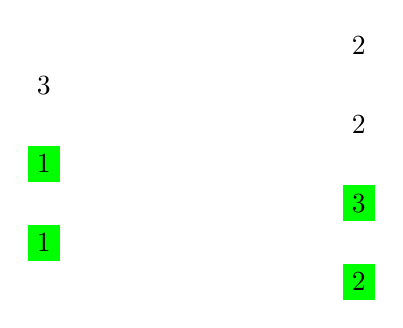
\begin{tikzpicture}[x=2cm]
                \tikzset{
                    sel/.style={fill=green}
                    ,drop/.style={fill=red}
                }
                \begin{scope}[yshift=.5cm,every node/.append style={rectangle}]
                    \node[sel](l1) at(0,0){1};
                    \node[sel](l2) at(0,1){1};
                    \node[](l3) at(0,2){3};
                \end{scope}
                
                \node[sel](r1) at(2,0){2};
                \node[sel](r2) at(2,1){3};
                \node[](r3) at(2,2){2};
                \node[](r4) at(2,3){2};
            
                \foreach \l \r in{
                    1/1%
                    ,2/2%
                    ,3/2,3/3,3/4%
                }{
                    \edge{l\l}{r\r};
                }
            \end{tikzpicture}    
        \end{column}
        \begin{column}{.5\textwidth}
            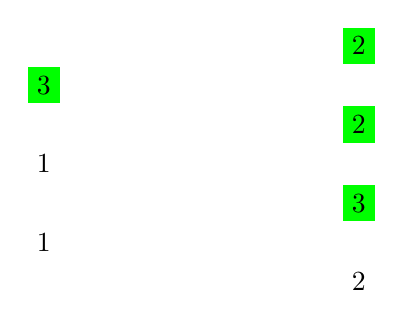
\begin{tikzpicture}[x=2cm]
                \tikzset{
                    sel/.style={fill=green}
                    ,drop/.style={fill=red}
                }
                \begin{scope}[yshift=.5cm,every node/.append style={rectangle}]
                    \node[](l1) at(0,0){1};
                    \node[](l2) at(0,1){1};
                    \node[sel](l3) at(0,2){3};
                \end{scope}
                
                \node[](r1) at(2,0){2};
                \node[sel](r2) at(2,1){3};
                \node[sel](r3) at(2,2){2};
                \node[sel](r4) at(2,3){2};
            
                \foreach \l \r in{
                    1/1%
                    ,2/2%
                    ,3/2,3/3,3/4%
                }{
                    \edge{l\l}{r\r};
                }
            \end{tikzpicture}    
        \end{column}
    \end{columns}
    \pause
    \begin{theorem}
        The Modified Greedy Algorithm is a $(1 - e^{-\frac{1}{2}})$-approximation.
    \end{theorem}
\end{frame}